\chapter{TO be checked what can be deleted or kept in other sections}
\section{Frame}


The most stringent requirement for the choice of the frame is to fit the \gls{oc}. So, I choose the smallest size of frame that could fit the \gls{oc} and have propellers commonly used for this size. So, it was a 330mm frame with 7 inch propeller to have a hub diameter of 152mm \ref{fig:330_7} (enough to fit the \gls{oc}). But this size was to large, so a smaller was chosen at the cost of smaller propeller. The efficiency  is reduced as the propeller need to rotate faster which mean higher \gls{kv}. So, a size of 275mm frame with 5 inch propeller was choosen with a hub diameter of 148mm \ref{fig:275_5.png}.

\begin{figure}[!ht]
    \centering
    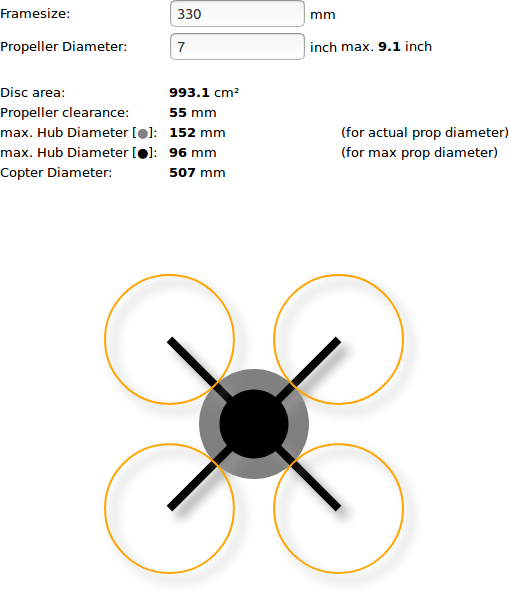
\includegraphics[width=.5\linewidth]{design/330_7.png}
    \caption{First choice of frame}
    \label{fig:330_7}
\end{figure}

\begin{figure}[!ht]
    \centering
    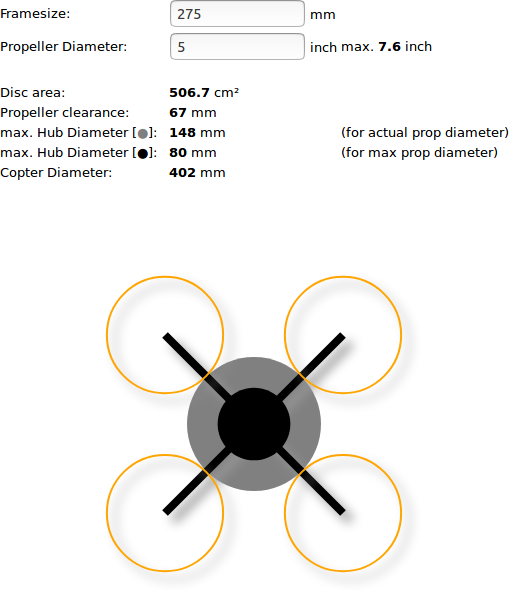
\includegraphics[width=.5\linewidth]{design/275_5.png}
    \caption{Second choice of frame}
    \label{fig:275_5.png}
\end{figure}

Three frame have been selected from these criteria a 330mm frame (\hyperref[fig:f330]{F330}) and two 275mm frame (\hyperref[fig:minibiggerracer]{Minibigger Racer} and \hyperref[fig:f2mito]{F2 Mito}).

\begin{figure}[!ht]
    \centering
    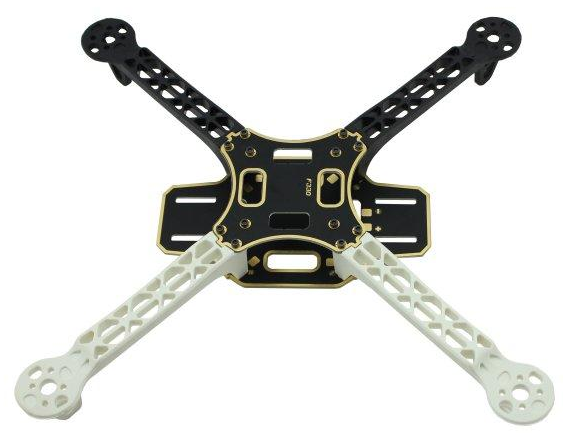
\includegraphics[width=.5\linewidth]{design/f330.png}
    \caption{\href{https://www.banggood.com/DJI-F330-4-Axis-RC-Quadcopter-Frame-Kit-Support-KK-MK-MWC-p-943370.html?rmmds=search&ID=48074&cur_warehouse=CN}{F330}}
    \label{fig:f330}
\end{figure}

\begin{figure}[!ht]
    \centering
    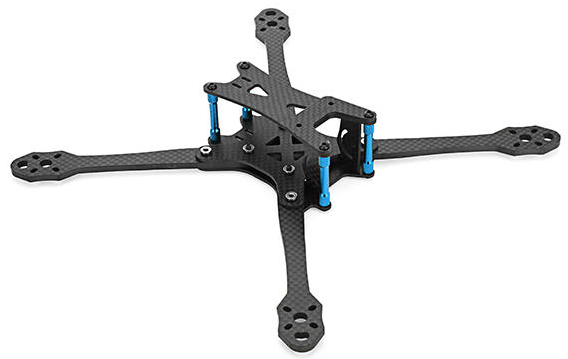
\includegraphics[width=.5\linewidth]{design/minibigger_racer.png}
    \caption{\href{https://www.banggood.com/Minibigger-Racer-255mm-275mm-Carbon-Fiber-4mm-Arm-RC-Drone-FPV-Racing-Frame-Kit-with-Wrench-Tools-p-1241634.html?rmmds=search&ID=228532758&cur_warehouse=CN}{Minibigger Racer}}
    \label{fig:minibiggerracer}
\end{figure}

\begin{figure}[!ht]
    \centering
    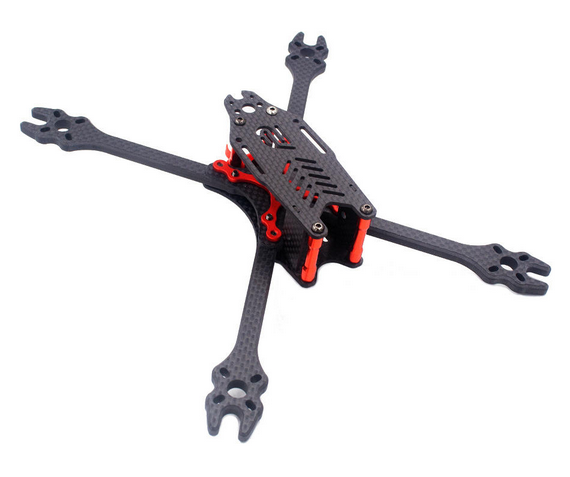
\includegraphics[width=.5\linewidth]{design/f2_mito.png}
    \caption{\href{https://www.banggood.com/F2-Mito-GS-Carbon-Fiber-195220250275mm-Freestyle-Stretch-X-Frame-Kit-for-RC-FPV-Racing-Drone-p-1319168.html?rmmds=search&ID=532758&cur_warehouse=CN}{F2 Mito}}
    \label{fig:f2mito}
\end{figure}

\section{Propellers}

As, the drone just a need a thrust-weight ratio of 2, the number of blades chosen is 2.

For the 330mm frame the propeller chosen was a \hyperref[fig:7045]{propeller 7045} and for the 275mm frame a \hyperref[fig:5030]{propeller 5030}.

\begin{figure}[!ht]
    \centering
    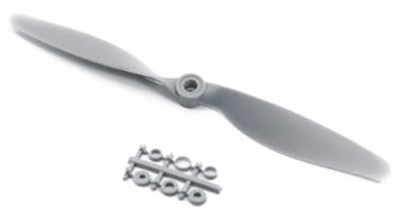
\includegraphics[width=.5\linewidth]{design/7045.png}
    \caption{\href{https://www.banggood.com/Style-7050-7x5-DD-Direct-Drive-Propeller-Blade-CW-CCW-For-RC-Airplane-p-1045332.html?rmmds=search&ID=45905&cur_warehouse=CN}{Propeller 7045}}
    \label{fig:7045}
\end{figure}

\begin{figure}[!ht]
    \centering
    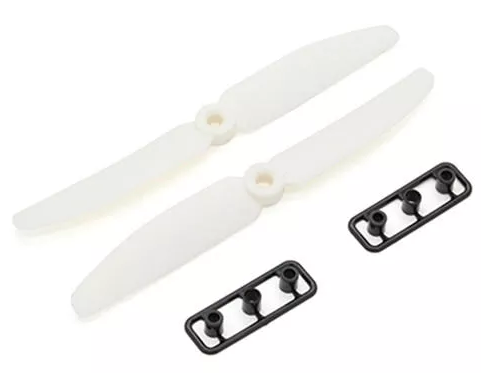
\includegraphics[width=.5\linewidth]{design/5030.png}
    \caption{\href{https://www.banggood.com/2pcs-WSX-5030-53-Inch-ABS-Propeller-White-CWCCW-for-RC-Drone-FPV-Racing-Multirotors-p-1387499.html?rmmds=search&cur_warehouse=CN}{Propeller 5030}}
    \label{fig:5030}
\end{figure}

\section{Motors}

Propeller adapter

\section{Battery}

\section{Power Distribution Board}

\section{Flight Controller}

\section{Radio Transmitter/Receiver}

\section{Miscellaneous}

\section{Weight}
